\documentclass[a4paper]{article}

\usepackage[english]{babel}
\usepackage[utf8]{inputenc}
\usepackage{amsmath}
\usepackage{graphicx}
\usepackage[colorinlistoftodos]{todonotes}
\usepackage{float}
\usepackage[margin=1 in]{geometry}
\usepackage{caption}
\usepackage[section]{placeins}

\title{Homework 3: \LaTeX{}}

\author{Goni Halevi}

\date{\today}

\begin{document}
\maketitle

\begin{abstract}
This morning, I ate a slice of whole wheat toast with almond butter, chia seeds, flax seeds, and some blueberries. And I drank coffee, of course.
\end{abstract}

\section{Lists}

\subsection{Things I Enjoyed About This Class}

\begin{itemize}
  \item Meeting and interacting with other Astro and Physics majors.
    \item Being able to do anything but Charman homework for two hours a week.
    \item Getting access to the lab. Everyone knows that the number of rooms and buildings that you have keycard access to directly signifies your success.
\end{itemize}

\subsection{Things I Did Not Like About This Class}

\begin{enumerate}
  \item I still feel like I don't know much IDL..... which is more my fault than yours, and obviously kind of expected since this is just a decal and not designed to make us all proficient programmers.
    \item Github.
    \item Github.
    \item Github.
    \item Github.
\end{enumerate}

\section{Euler-Lagrange Equation}
$$\sum_{j=1}^{n} (-1)^j\partial^j_{\mu_{1}...\mu_{j}}\bigg(\frac{\partial\mathcal{L}}{\partial f_{i,\mu_{1}...\mu{j}}}\bigg) $$
where summation over the \(\mu_{1}...\mu_{j}\) is implied according to Einstein notation.

\section{Table}
\begin{table}[H]
\center
\begin{tabular} {|l|c|r|} 
\hline
Favorite Foods & Favorite Bands & Favorite IDL Commands \\\hline
Almonds & The Shins & tvscl \\
Avocado & Real Estate & mrdfits \\
Blueberries & Local Natives & plot \\\hline
\end{tabular}
\caption{\label{tab:widgets}My favorite genres of music are indie folk or alternative rock, but I generally like anything mellow and dreamy with good vocals.}
\end{table}


\section{My Pretty Plot}
\begin{figure}[!htb]
  \centering
  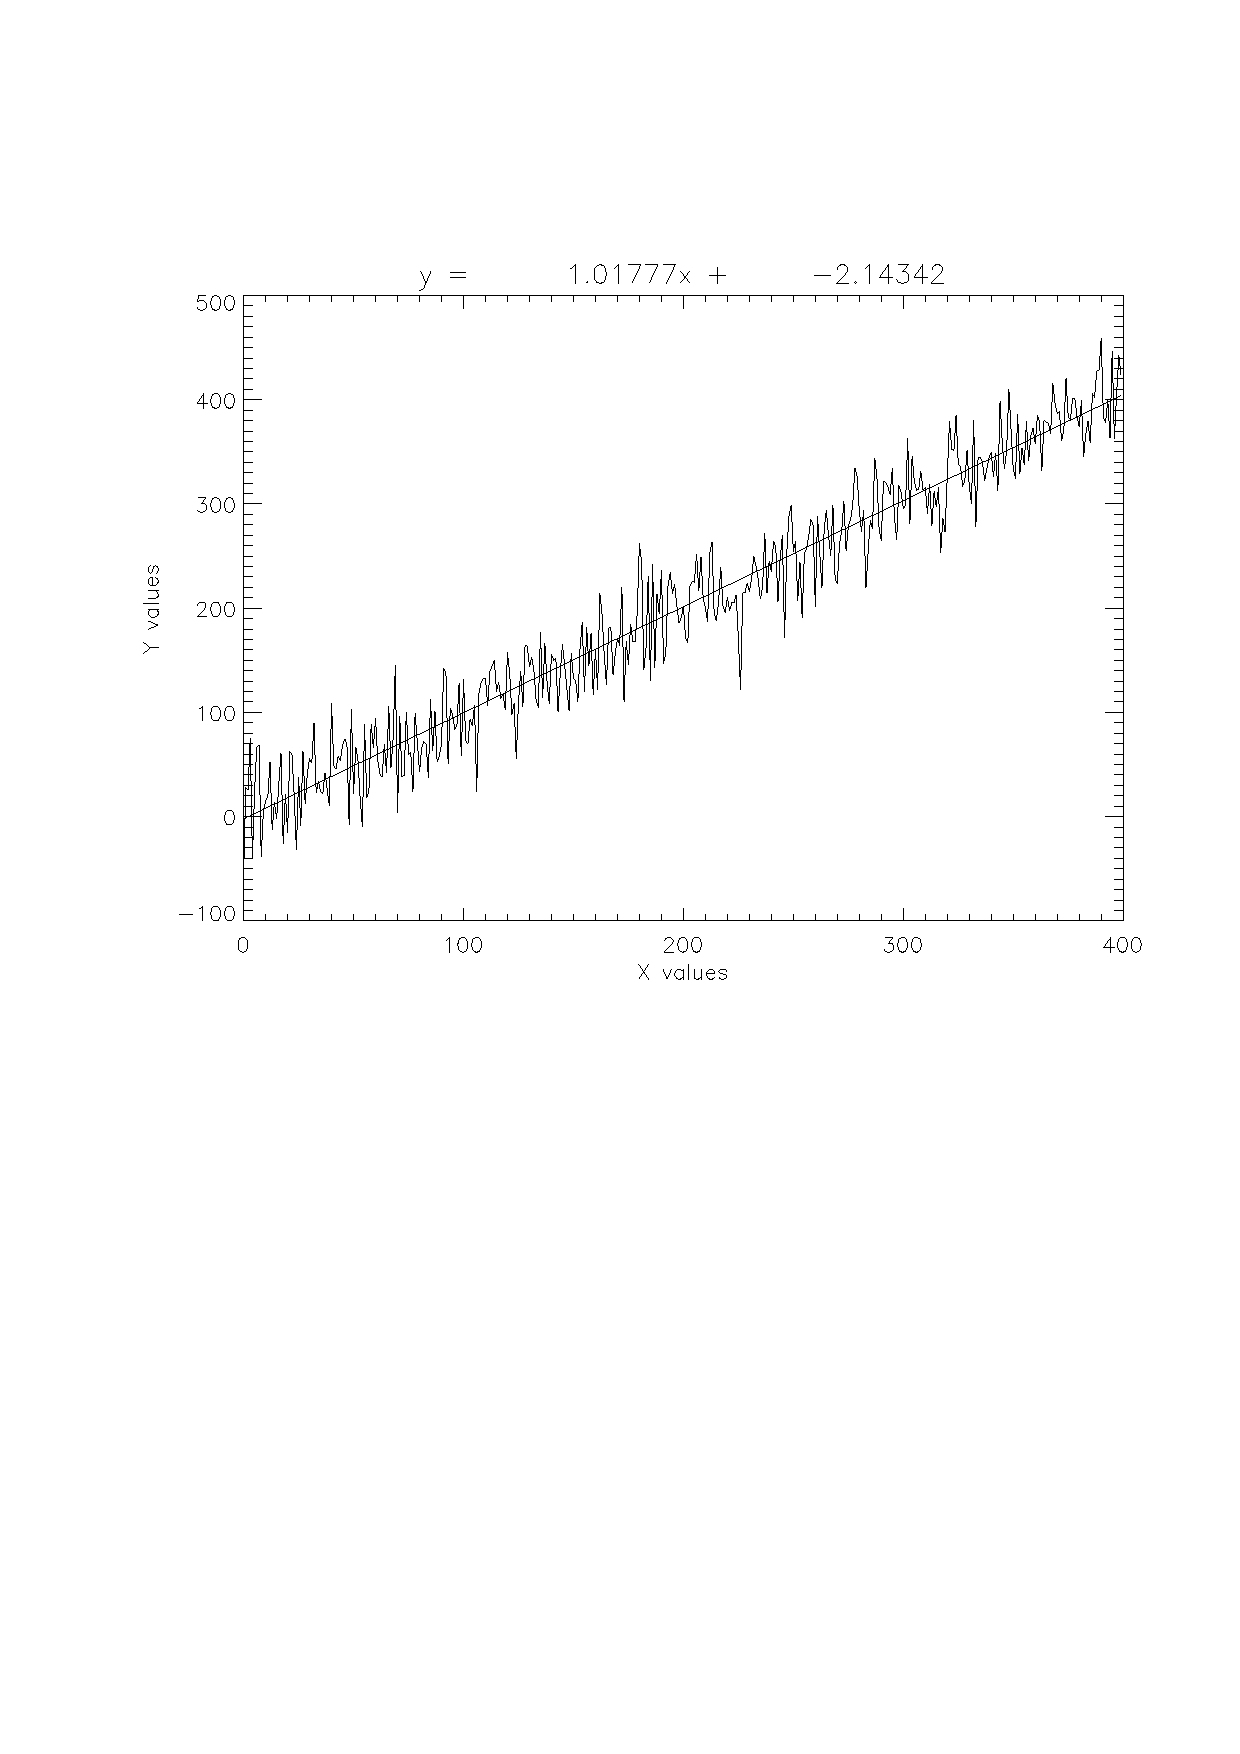
\includegraphics[width=0.7\textwidth]{tut6.jpg}
  \captionsetup{width=0.7\textwidth}
   \caption{This plot is from my least-squares regression tutorial. I like it because I used stars for the scatterplot points and it came out looking nice. I struggled to scale my axes correctly, but once I figured that out, everything about that tutorial was simple and applicable.}
\end{figure}


\section{My Favorite Things}
\begin{figure}[!htb]
\centering
\begin{minipage}[!htb]{0.42\linewidth}
\includegraphics[width=\textwidth]{starz.jpg}
\caption{A crappy picture of the stars from Lick Observatory}
\label{fig:minipage1}
\end{minipage}
\quad
\begin{minipage}[!htb]{0.45\linewidth}
\includegraphics[width=\textwidth]{catz.jpg}
\caption{Really cute cats at Lick Observatory}
\label{fig:minipage2}
\end{minipage}
\end{figure}


\end{document}
